% Figure includes generated in the nature-figure step. Widths match set_paper_placement() in each gen_fig_*.py.
% Data figures: figures/gen_fig_*.py (matplotlib, Nature style); tikz_q1_set_logic: figures/tikz_q1_set_logic.tex.
% HTML diagrams fig_roadmap / fig_arch_fusion are produced in the next step (paper-figure-html).

% ---------------- Problem 1
\begin{figure}[H]
  \centering
  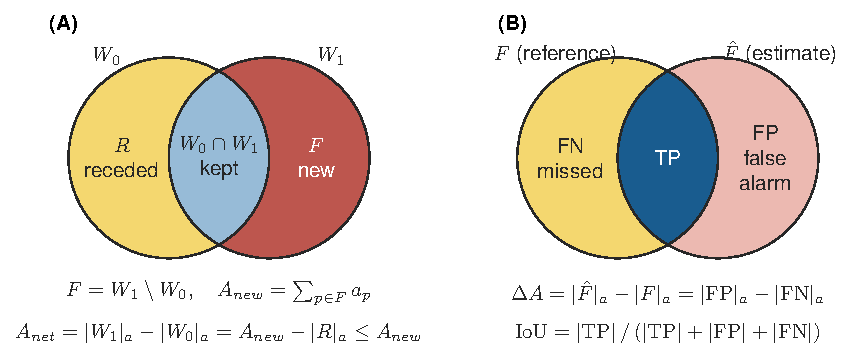
\includegraphics[width=0.90\textwidth]{figures/tikz_q1_set_logic.pdf}
  \caption{Set logic of the area definitions. (a) Pre-flood water $W_0$, flood-time water $W_1$, new inundation $F=W_1\setminus W_0$ and receded water $R=W_0\setminus W_1$; the net change $A_{net}=A_{new}-|R|_a$ can never exceed $A_{new}$. (b) Reference $F$ versus estimate $\hat F$: the area error equals $|\mathrm{FP}|_a-|\mathrm{FN}|_a$, so false alarms and misses can cancel in the total.}
  \label{fig:q1_set_logic}
\end{figure}

\begin{figure}[H]
  \centering
  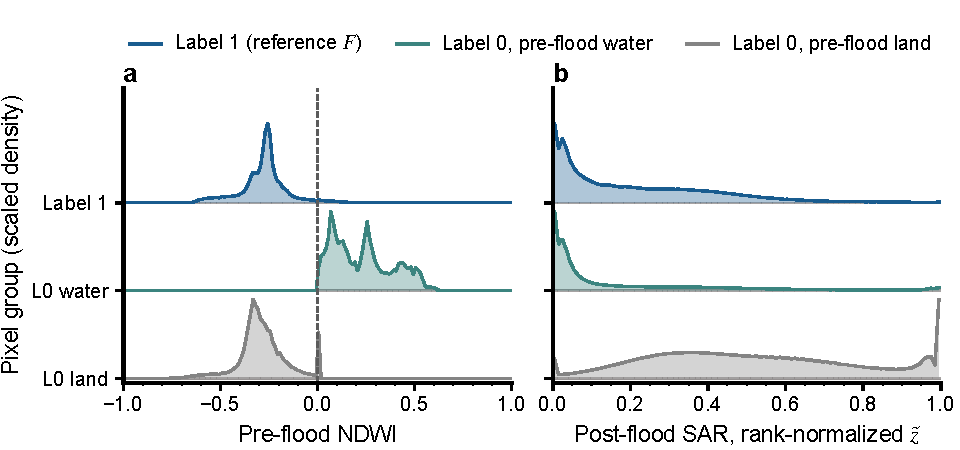
\includegraphics[width=0.95\textwidth]{figures/fig_q1_label_semantics.pdf}
  \caption{Label-semantics test on all 65,491,966 valid pixels of the 1000 official tiles. (a) Pre-flood NDWI and (b) rank-normalized post-flood SAR brightness for three pixel groups; densities are scaled to equal height. Only 2.37\% of label-1 pixels have NDWI\,$>0$ before the event, while 70.1\% of pre-flood water pixels labelled 0 are still SAR-dark, so the labels mark new inundation and exclude permanent water.}
  \label{fig:q1_label_semantics}
\end{figure}

\begin{figure}[H]
  \centering
  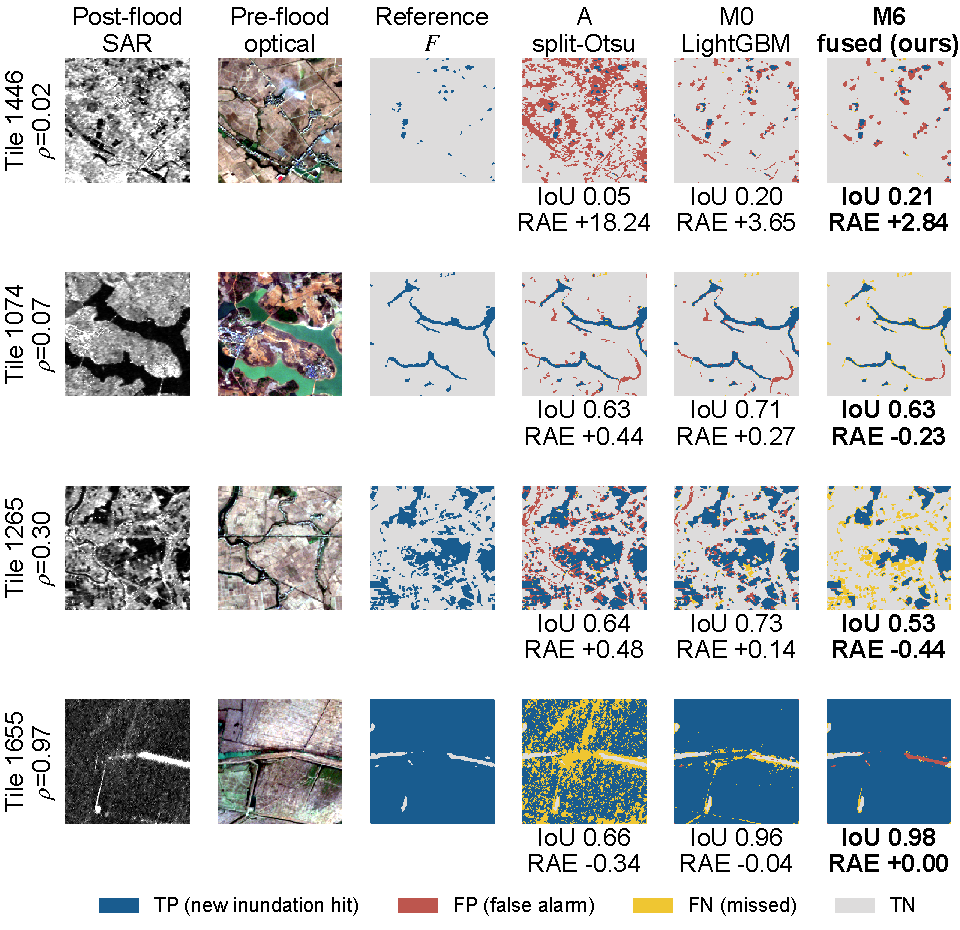
\includegraphics[width=0.98\textwidth]{figures/fig_q1_visual_cmp.pdf}
  \caption{Held-out predictions on four official tiles of increasing flood share $\rho$ (tiles chosen in the coding step). Columns 4--6 show the confusion map of each model against the reference; per-tile IoU and relative area error (RAE) are given under each map. Every tile is predicted by the model of the spatial fold in which it was a test tile.}
  \label{fig:q1_visual_cmp}
\end{figure}

\begin{figure}[H]
  \centering
  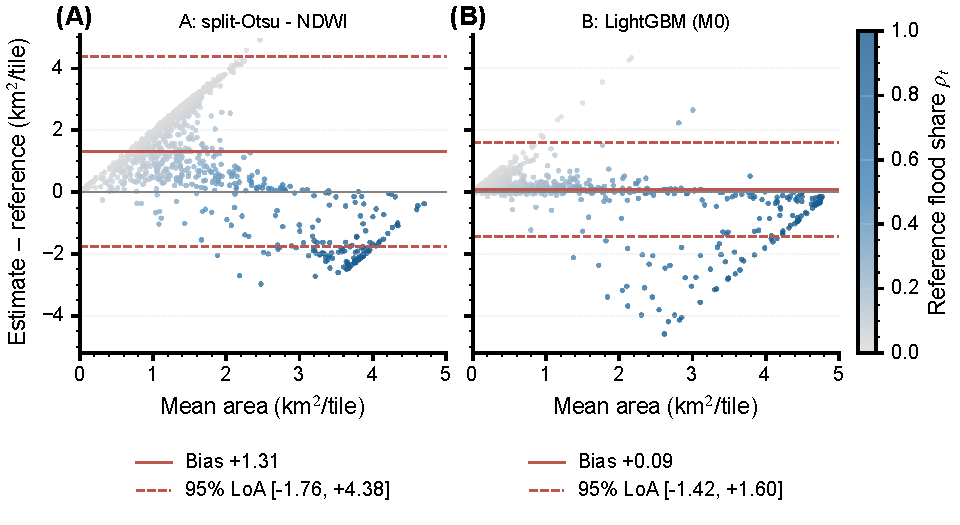
\includegraphics[width=0.95\textwidth]{figures/fig_q1_area_agreement.pdf}
  \caption{Bland--Altman agreement of the tile new-inundation area over the 1000 held-out tiles (blocked 5-fold CV). (a) Baseline A (split-Otsu minus NDWI) over-estimates by $+1.31$\,km$^2$ per tile on average; (b) LightGBM M0 has bias $+0.09$\,km$^2$ and 95\% limits of agreement $[-1.42,+1.60]$\,km$^2$. Colour is the reference flood share of the tile.}
  \label{fig:q1_area_agreement}
\end{figure}

\begin{figure}[H]
  \centering
  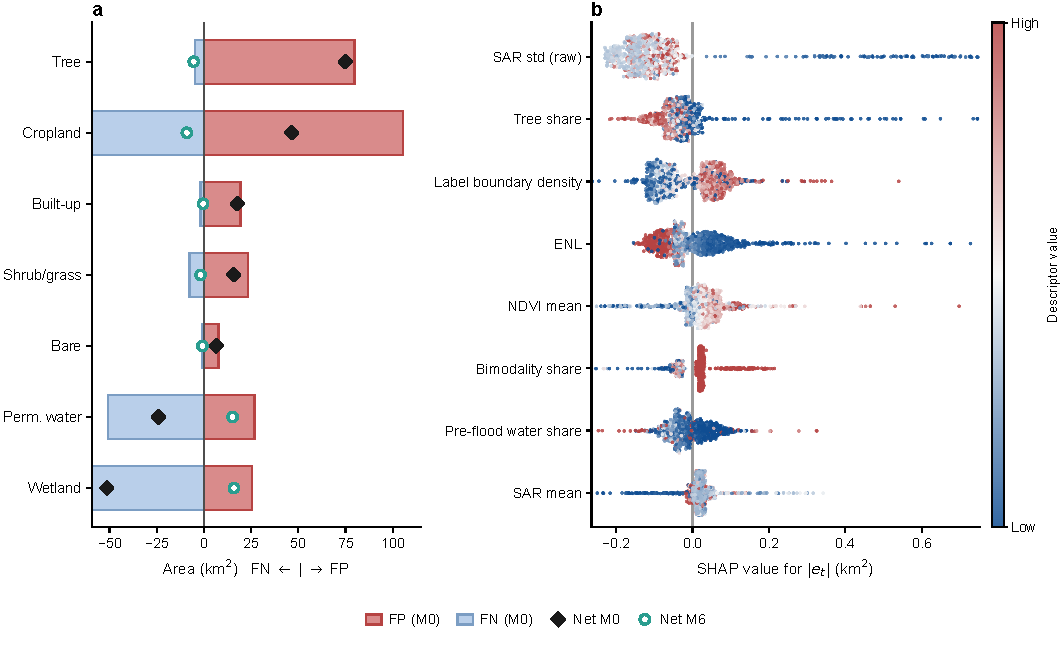
\includegraphics[width=0.98\textwidth]{figures/fig_q1_error_drivers.pdf}
  \caption{Error structure of the Q1 model. (a) False-positive and false-negative area of LightGBM M0 by pre-flood ESA WorldCover class, with the net error of M0 and of the final fused model M6 (Q2); the per-class sums satisfy $\sum(\mathrm{FP}-\mathrm{FN})=\Delta A$. (b) TreeSHAP values of the eight strongest tile descriptors for the out-of-fold regressor of $|e_t|$ (OOF $R^2=0.417$); colour is the descriptor value (5--95\% scaled).}
  \label{fig:q1_error_drivers}
\end{figure}

% ---------------- Problem 2
\begin{figure}[H]
  \centering
  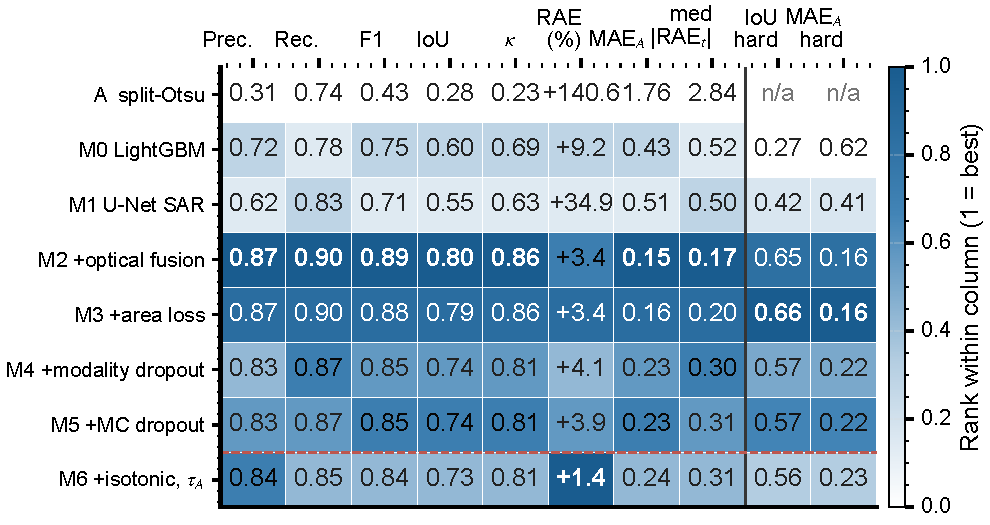
\includegraphics[width=0.98\textwidth]{figures/fig_q2_model_compare.pdf}
  \caption{All models evaluated on the same 1000 held-out tiles and, in the last two columns, on the 397 tiles that were hard for the Q1 model. Cell text is the metric value; colour is the rank within the column (1 = best). RAE is given in percent. Baseline A was not run on the hard subset.}
  \label{fig:q2_model_compare}
\end{figure}

\begin{figure}[H]
  \centering
  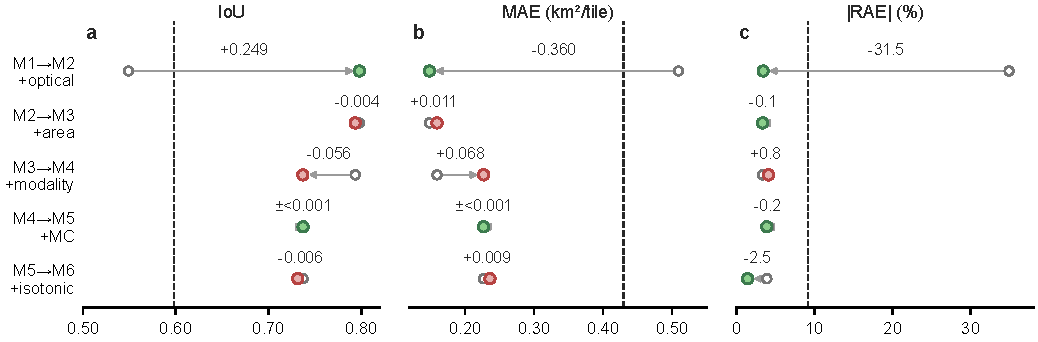
\includegraphics[width=0.98\textwidth]{figures/fig_q2_ablation.pdf}
  \caption{Ablation from the SAR-only U-Net (M1) to the final model (M6): change of (a) IoU, (b) tile mean absolute area error and (c) absolute total relative area error caused by each added component. The dashed line is LightGBM M0. Optical fusion gives the largest gain; modality dropout costs accuracy in-domain but is kept for the optics-free transfer of Q3; isotonic calibration with the area-preserving threshold reduces $|$RAE$|$ from 3.9\% to 1.45\%.}
  \label{fig:q2_ablation}
\end{figure}

\begin{figure}[H]
  \centering
  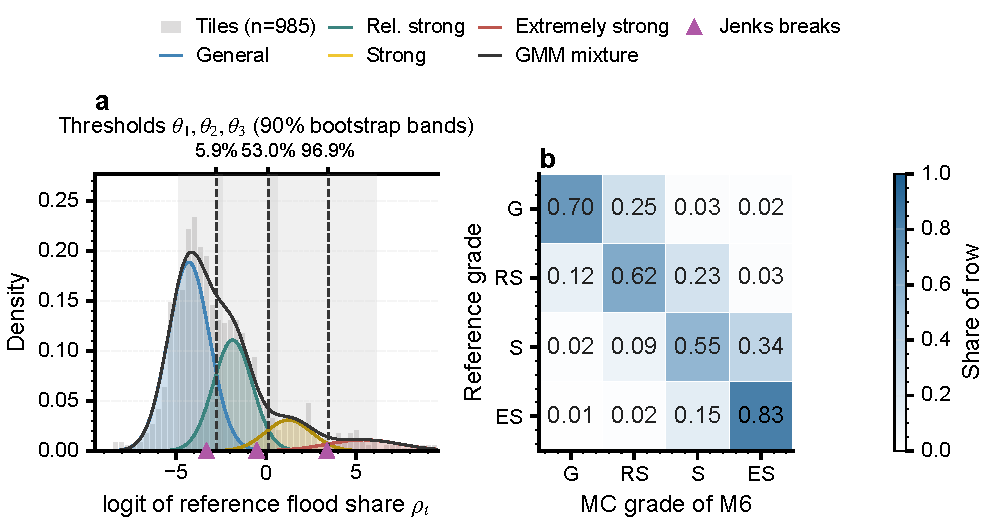
\includegraphics[width=0.98\textwidth]{figures/fig_q2_grading.pdf}
  \caption{Data-based four-level grading. (a) Histogram of $\operatorname{logit}\rho_t$ for the 985 non-empty reference tiles with the four-component Gaussian mixture; dashed lines are the Bayes thresholds $\theta=(5.9\%,53.0\%,96.9\%)$, grey bands their 90\% block-bootstrap intervals, triangles the Jenks breaks. (b) Reference grade versus the Monte Carlo grade of M6 (M = 2000 residual and threshold draws), row-normalized. G, RS, S, ES: general, relatively strong, strong, extremely strong.}
  \label{fig:q2_grading}
\end{figure}

% ---------------- Problem 3
\begin{figure}[H]
  \centering
  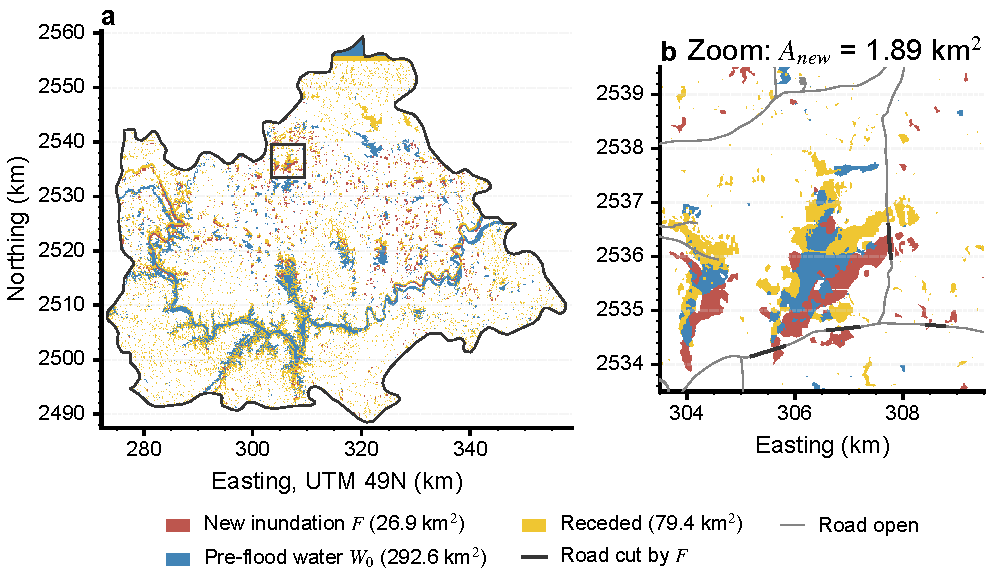
\includegraphics[width=0.98\textwidth]{figures/fig_q3_newflood_map.pdf}
  \caption{New inundation in Hengzhou on 16 July 2026 from co-registered Sentinel-1 and the transferred M6 model with physics guards. (a) Whole city, shown on 100\,m display cells (a cell is coloured if it contains any pixel of the class); (b) the $6\times6$\,km window with the largest new area at 10\,m resolution, with roads cut by $F$. The horizontal band near northing 2555\,km is an artefact of the co-registration edge in $W_0$ and $R$; it contains no new inundation.}
  \label{fig:q3_newflood_map}
\end{figure}

\begin{figure}[H]
  \centering
  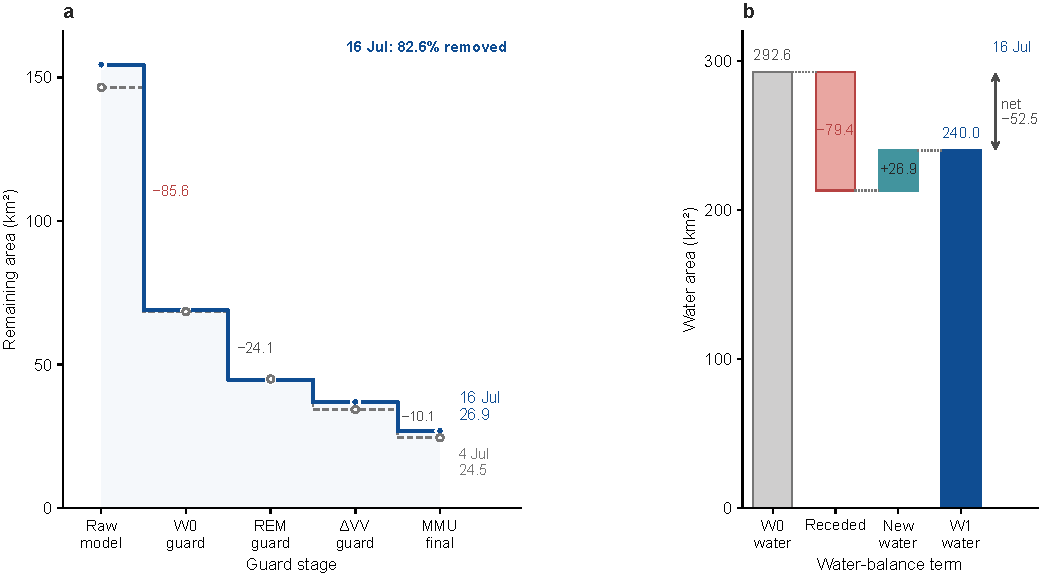
\includegraphics[width=0.95\textwidth]{figures/fig_q3_area_budget.pdf}
  \caption{Area budget of Hengzhou for the two flood dates. (a) Guard cascade from the raw model mask to the final new inundation; the guards remove 83.3\% (07-04) and 82.6\% (07-16) of the model area. (b) Water-balance terms: the net change is negative on both dates because water receded after the wet 27 June baseline, while $A_{new}=24.5$ and $26.9$\,km$^2$.}
  \label{fig:q3_area_budget}
\end{figure}

\begin{figure}[H]
  \centering
  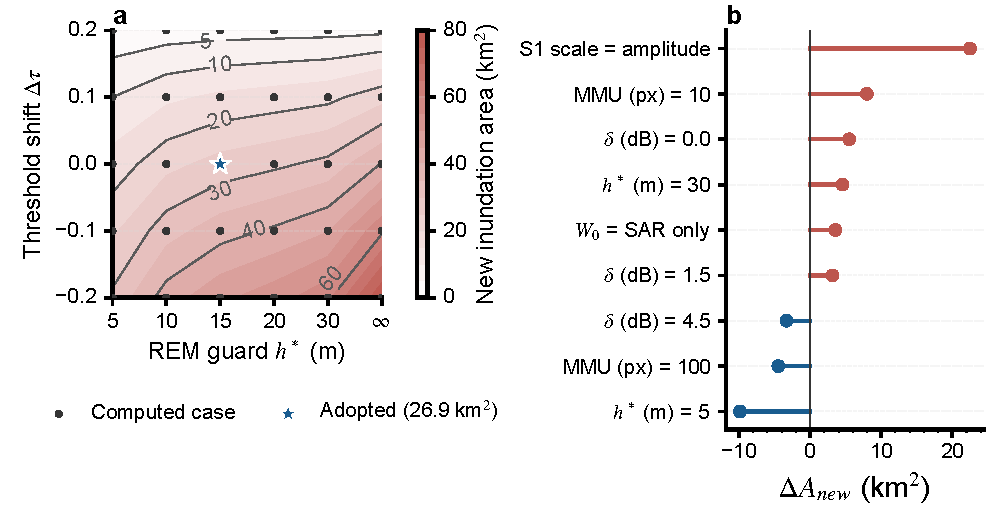
\includegraphics[width=0.98\textwidth]{figures/fig_q3_threshold_surface.pdf}
  \caption{Sensitivity of the Hengzhou new-inundation area (07-16). (a) Response surface over the probability-threshold shift $\Delta\tau$ and the REM guard $h^*$ (30 full re-computations, dots); the star is the adopted setting. (b) One-at-a-time changes of the change-guard margin $\delta$, the $W_0$ definition, the SAR scale, the minimum mapping unit and $h^*$. The grade remains ``general'' in every case because all $\rho<\theta_1=5.9\%$.}
  \label{fig:q3_threshold_surface}
\end{figure}

% ---------------- Problem 4
\begin{figure}[H]
  \centering
  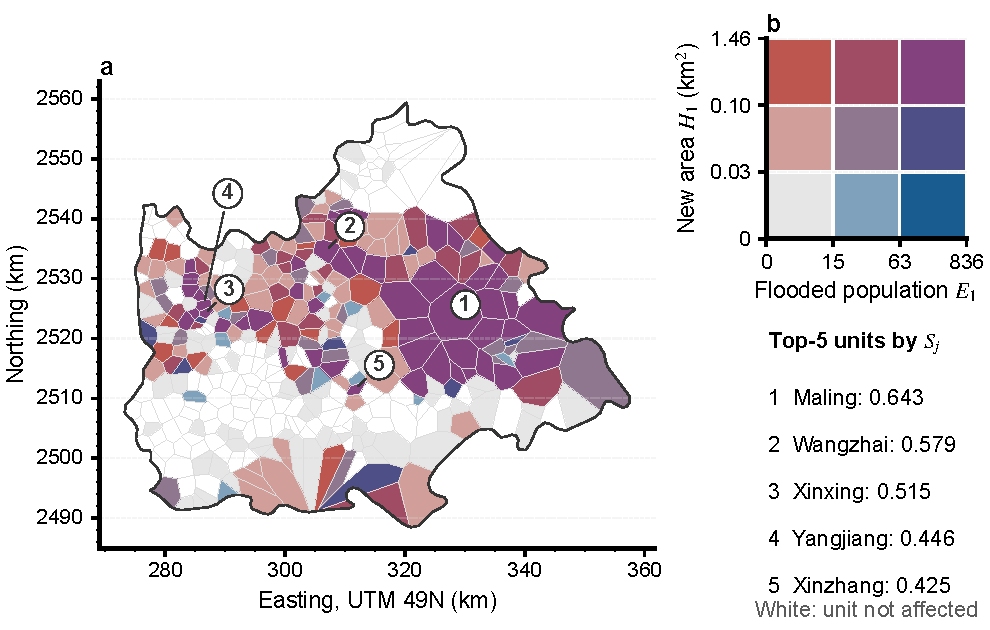
\includegraphics[width=0.98\textwidth]{figures/fig_q4_risk_map.pdf}
  \caption{Bivariate map of the 393 place-catchment units of Hengzhou. (a) Hazard (new inundation area $H_1$) crossed with exposure (flooded population $E_1$, WorldPop 2020), each split at the tertiles of the non-zero values of the 259 affected units; numbers mark the five units with the highest TOPSIS index $S_j$. (b) Colour key with class limits. Names are given in pinyin.}
  \label{fig:q4_risk_map}
\end{figure}

\begin{figure}[H]
  \centering
  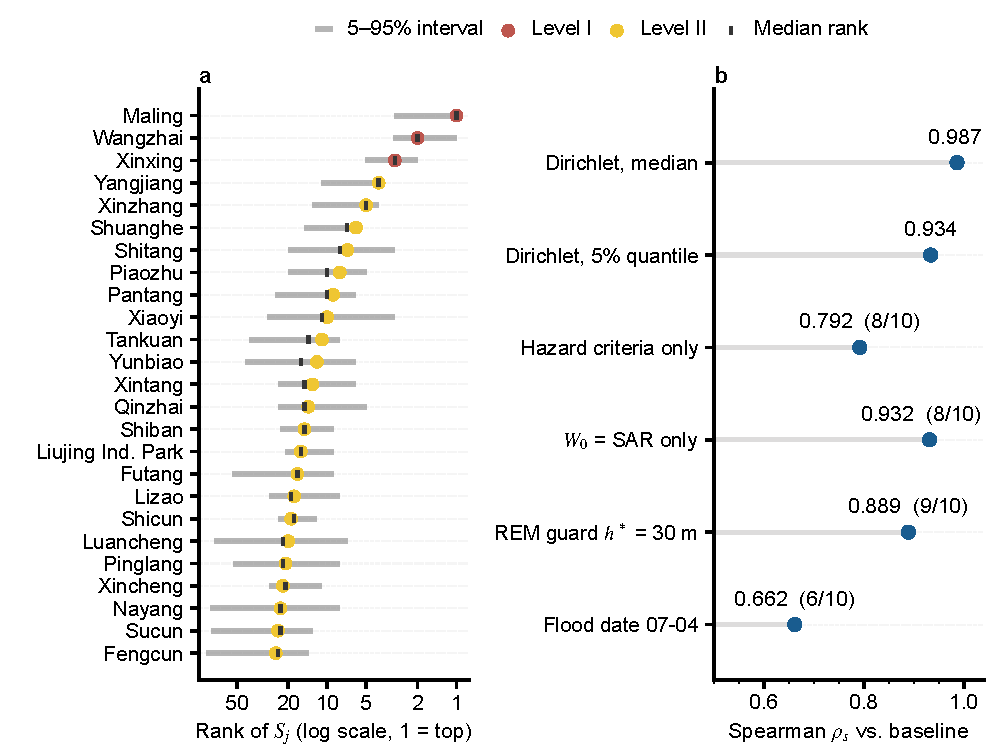
\includegraphics[width=0.98\textwidth]{figures/fig_q4_rank_robustness.pdf}
  \caption{Robustness of the unit ranking. (a) Baseline rank (colour = Jenks level), median and 5--95\% interval of the rank under Dirichlet perturbation of the indicator weights (M = 2000) for the 25 highest-ranked units. (b) Spearman correlation with the baseline ranking for perturbed weights, hazard-only weights and three alternative Q3 inputs; brackets give the overlap of the top-10 sets.}
  \label{fig:q4_rank_robustness}
\end{figure}

% ---------------- Problem 5
\begin{figure}[H]
  \centering
  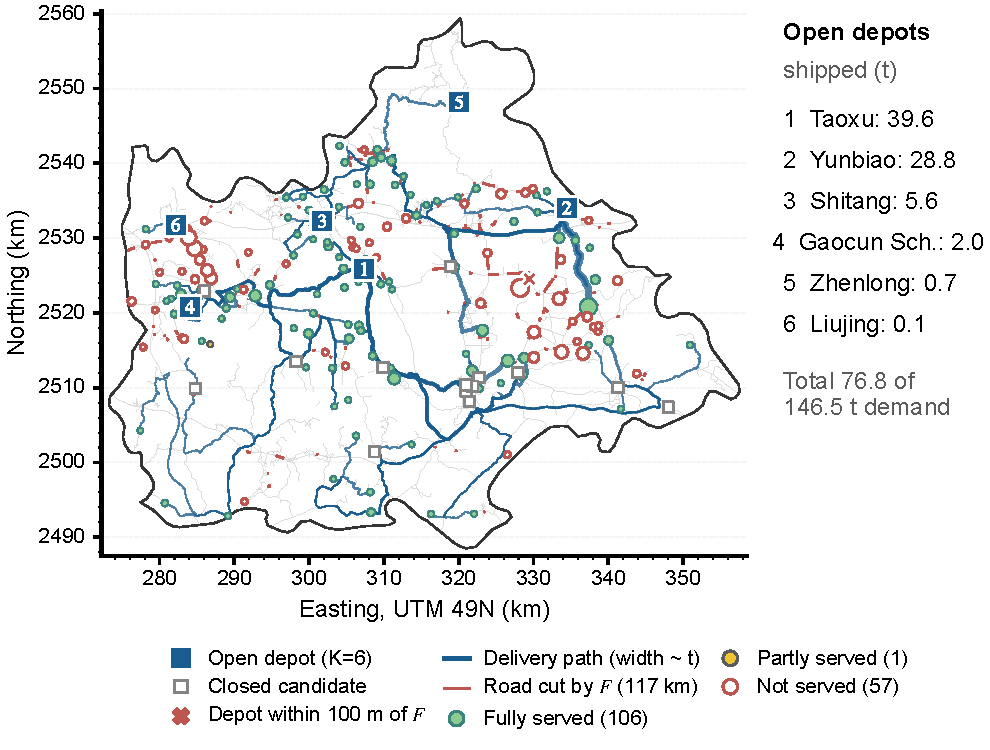
\includegraphics[width=0.98\textwidth]{figures/fig_q5_route_alloc.pdf}
  \caption{Recommended relief plan for 16 July 2026 on the flood-cut road network (lexicographic MILP, HiGHS, optimal). Numbered squares are the six open depots, ordered by shipped tonnage; line width of a delivery path is proportional to its tonnage. Of 164 demand units, 57 have no admissible depot within the time limit after the flood cut and remain unserved; supply capacity is not binding.}
  \label{fig:q5_route_alloc}
\end{figure}

\begin{figure}[H]
  \centering
  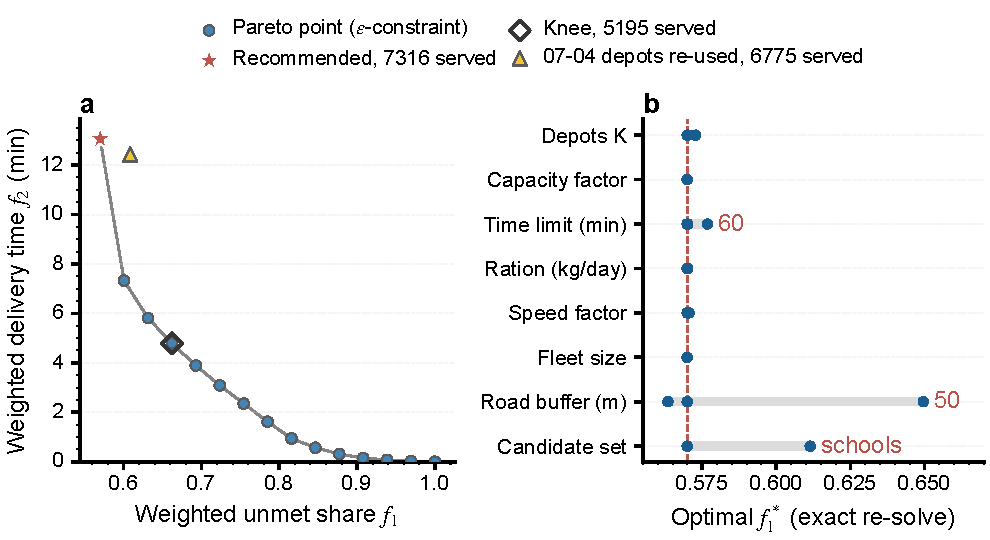
\includegraphics[width=0.98\textwidth]{figures/fig_q5_pareto.pdf}
  \caption{(a) $\varepsilon$-constraint Pareto front of the priority-weighted unmet share $f_1$ and the priority-weighted delivery time $f_2$ (15 exact solves) with the recommended plan, the knee point and the 4 July depot set re-optimized under 16 July inputs (value of information $+0.039$ in $f_1$). (b) Optimal $f_1^*$ in 30 one-at-a-time exact re-solves; dashed line = recommended plan. Only the road-flood buffer and the candidate set move $f_1^*$ by more than 0.005.}
  \label{fig:q5_pareto}
\end{figure}
